\documentclass[12pt,letterpaper,noanswers]{exam}
\usepackage[usenames,dvipsnames,svgnames,table]{xcolor}
\usepackage[margin=0.9in]{geometry}
\renewcommand{\familydefault}{\sfdefault}
\usepackage{multicol}
\pagestyle{head}
\header{AM 108 Class 18}{}{Poincar\'e map}
\runningheadrule
\headrule
\usepackage{graphicx} % more modern
\usepackage{amsmath} 
\usepackage{amssymb} 
\usepackage{hyperref}
\usepackage{tcolorbox}

\begin{document}
 \pdfpageheight 11in 
  \pdfpagewidth 8.5in

\noindent 




\begin{itemize}

   
    \item Fill out the project preference form (it is on Gradescope - upload it there when done). 
    \item There will not be a pre-class assignment for Friday; there is a problem set.
    \item There will be a skill check in class on Friday.  The problem info is below.
 \item Problem set 07 is due Friday October 23rd.
\end{itemize}

\hrule
\vspace{0.2cm}



\noindent\textbf{Teams}

\begin{multicols}{2}
1. 

\end{multicols}

\noindent \textbf{Teams 5 and 6}: Post screenshots of your work to the course Google Drive today.  Include words, labels, and other short notes that might make those solutions useful to you or your classmates.  Find the link in Canvas (or here: \url{https://drive.google.com/drive/u/0/folders/1GcpwvKHD4tMecpFQ4lNxN_r5Ylj7YHbd})

\vspace{0.2cm}

\hrule
\vspace{0.2cm}

\noindent\textbf{Polls}


\vspace{0.2cm}

\hrule
\vspace{0.2cm}

\noindent\textbf{Big picture}

We are looking at how bifurcations manifest in 2d systems.  The saddle-node, transcritical, and pitchfork bifurcations generalize from occuring when $f'(x^*) = 0$ to occurring when $\left.Df\right\vert_{\underline x^*}$ (the Jacobian matrix evaluated at the fixed point) has a zero eigenvalue.

We have some new bifurcations that can occur in 2d systems and don't exist in 1d systems.  The Hopf bifurcation is one of these and is a bifurcation in which a fixed point changes stability and a limit cycle is born/annihilated.  


\vspace{0.2cm}
\hrule
\vspace{0.2cm}


\noindent \textbf{Extra vocabulary / extra facts:}
\begin{tcolorbox}
Identifying bifurcations in higher dimensional systems is an important aspect of determining the possible long term behaviors in systems with a parameter.
\begin{itemize}
\itemsep0em
    \item When a single eigenvalue crosses zero as a parameter changes, that corresponds to a saddle-node, a transcritical, or a pitchfork bifurcation.  Note: The presence of a zero eigenvalue means the determinant of the Jacobian matrix will be zero, $\det\left.Df\right\vert_{\underline x^*} = 0$.
    \item When the real part of a complex conjugate pair of eigenvalues crosses zero as a parameter changes, that corresponds to a Hopf bifurcation.  In a 2D system, the determinant is positive and the trace is zero when this happens.
\end{itemize}

A Hopf bifurcation in which a stable limit cycle is born is called \textbf{supercritical}.  When an unstable limit cycle is born the bifurcation is \textbf{subcritical}.
\end{tcolorbox}

\vspace{0.2cm}

\hrule
\vspace{0.2cm}

\noindent\textbf{Your Questions}
\begin{enumerate}
    \item With the ``ghost'' region / bottleneck that occurs when a parameter value is close to a saddle-node bifurcation:
    \begin{enumerate}
        \item why does it happen / how does it work?
        \item once the fixed points are destroyed in the bifurcation, is the vector field smooth?
        \item does this slow region stay where the fixed points were, or does it move in phase space?
    \end{enumerate}
    \item How do these bifurcation differ from 1d?
    \begin{enumerate}
        \item Can the $x$ and $y$ variables be equally involved in the bifurcation?
        \item What if there are parameters in both equations?
        \item What if there are multiple parameters in the system?
    \end{enumerate}
    \item How do the eigenvalue plots relate to the phase portrait pictures of the bifurcation?
    \item How similar is the pitchfork bifurcation to a saddle-node / how are they related?
    \item In the pitchfork bifurcation example ($\dot x = a x - x^3, \dot y = -y$) there was a fixed point at the origin.  Why did Steve plot two points on the eigenvalue plot?
    \item What is a degenerate Hopf bifurcation?  (In the text, Steve gives the example $\ddot x + \mu \dot x + \sin x = 0$.)
\end{enumerate}

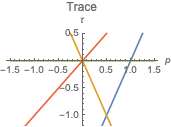
\includegraphics{img/C22-2019-10-28p1.png}
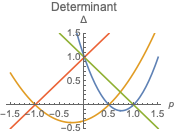
\includegraphics{img/C22-2019-10-28p2.png}



\vspace{0.2cm}

\hrule
\vspace{0.2cm}

\noindent\textbf{Skill Check C19 practice}
\begin{questions}
\item Retake of skill check C16: 


\item Consider the system 
\begin{align*}
\dot x &= \mu x + y - x^3 \\
\dot y &= -x+\mu y - 2y^3.
\end{align*}

This system has a fixed point at $(0, 0)$.  For that fixed point, a Hopf bifurcation occurs at some value of $\mu$.  Identify the bifurcation value, showing your mathematical steps.


\end{questions}

\framebox(200,50){\quad $\mu=$  \hfill}

\vspace{0.2cm}

\hrule
\vspace{0.2cm}

\noindent\textbf{Skill check C19 practice solution}

To locate the Hopf bifurcation, I want to classify the fixed point and identify when it changes stability (transitioning from a stable spiral to an unstable spiral).  At the point of bifurcation, the corresponding linear system will have a linear center.  The actual behavior of the nonlinear system is harder to determine and not something I need to figure out.

To classify the fixed point, I'll start by finding the Jacobian:

$\left(\begin{array}{c c} \mu - 3x^2 & 1 \\ -1 & \mu - 6y^2  \end{array}\right)$. At $(0,0)$, this is $\left(\begin{array}{c c} \mu  & 1 \\ -1 & \mu  \end{array}\right)$

The trace is $\tau = 2\mu$ and the determinant is $\Delta = 1+\mu^2$.  The determinant is positive for all values of $\mu$ (I need to check the sign of the determinant because when $\tau = 0$ and $\Delta < 0$ I have a saddle point, while when $\tau = 0$ and $\Delta > 0$, the linearized system has a linear center, i.e. a Hopf bifurcation).  $\tau = 0$ and $\Delta>0$ when $\mu = 0$, so the Hopf bifurcation occurs at $\mu = 0$. 

\vspace{0.2cm}

\hrule
\vspace{0.2cm}


\vspace{0.2cm}

\hrule
\vspace{0.2cm}
\noindent\textbf{Questions}

\noindent \ \ 0.  Discuss your breakfast preferences with the other members of your team (and write your names on the slide).

\begin{questions}
\question (8.1.6) Consider the system
\begin{align*}
\dot{x} = &\ y - 2x \\
\dot{y} = &\ \mu+x^2-y.
\end{align*}
\begin{parts}
\item Sketch the nullclines.
\item Find and classify the bifurcations that occur as $\mu$ varies.
\item Show that at the point of bifurcation the $\dot{x}=0$ and $\dot{y}=0$ nullclines are tangent.  
\item Do you expect this to usually be true for a saddle-node bifurcation?  What about for a transcritical or pitchfork bifurcation?
\end{parts}

\question (8.2.8) Consider the dimensionless predator-prey system:
\begin{align*}
\dot{x} = &\ x(x(1-x)-y) \\
\dot{y} = &\ y(x-a), \quad a>0.
\end{align*}
\begin{parts}
\item Which variable is representing prey, and which predators?
\item Find the fixed points of this system. (You can use Mathematica or do this by hand)
\item Determine the stability of these fixed points.  (You can use Mathematica or do this by hand)  \emph{The trace and determinant will be sufficient to classify two of the points.  For the third fixed point, drawing the nullclines may help you classify it.  Note that your classification will include different cases for different ranges of $a$.}
\item Make a variation on a bifurcation diagram by showing the locations of the fixed points: plot the $x$ value associated with each fixed point vs $a$ for $0 < a < 2$.  Used dashed lines for unstable or saddle points and solid lines for stable points.
\item What type of bifurcation occurs when $a=1$?  What about when $a = \frac{1}{2}$?
\item Estimate the frequency of limit cycle oscillations for $a$ very close to the bifurcation.
\item Does the Hopf bifurcation appear to be supercritical or subcritical?  

To allow you to see the direction of forward time, the cyan curve corresponds to time $0$ to $50$ of a forward integration, and the black curve to time $50$ to $400$.  The $a$ value is given in the caption of each plot.

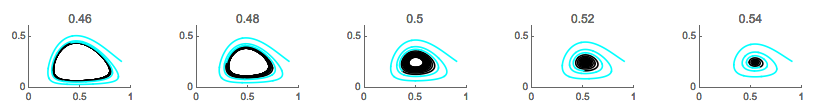
\includegraphics[width=6in]{img/S19C17p1.png}

\end{parts}

\end{questions}

\eject

1: a: The $\dot{x} = 0$ nullcline is in black and the $\dot{y} = 0$ nullcline is in blue for three different values of $\mu$.  These values
are below, at, and above the bifurcation point.


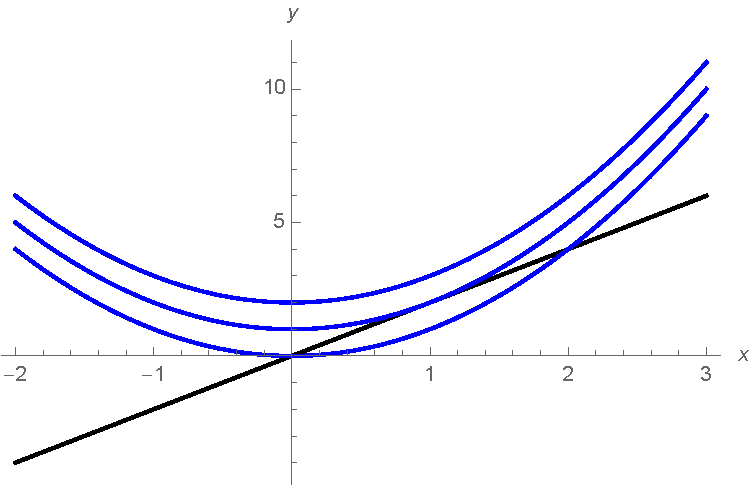
\includegraphics[width=2.5in]{img/C15nullclines.pdf}


b: To find and classify the bifurcations we need to identify the fixed points and find where the number of fixed points changes.
We can see from the nullclines that the black and blue lines intersect in two places for some values of $\mu$, and as $\mu$ increases
they intersect at a single point and then no points.  This means there's a saddle-node bifurcation.  So I've classified the bifurcation just
from looking at the nullcline picture.  To find the bifurcation, I suppose I need to find the point where there's just one fixed point, or, I can
find one of the fixed points and identify where it changes stability.  Either option would work.

At the fixed points $y = 2x$ and $y = \mu + x^2$ because $y-2x = 0$ and $\mu + x^2 - y = 0$.
This means $2x = \mu + x^2$ so $x^2 - 2x + \mu = 0$.  Using the quadratic formula,
\[x_\pm = 1 \pm \frac{1}{2} \sqrt{4 - 4\mu} = 1\pm \sqrt{1 - \mu}.\]
So there is just a single fixed point when $\mu = 1$ and for $\mu >1$ there are no fixed points.  Thus the bifurcation occurs
when $\mu = 1$ % at the point $(1, 2)$.

c: The slope of the $\dot{x} = 0$ nullcline of $y = 2x$ is $2$.  We want to show the other nullcline has the same slope at the point
of bifurcation.  The other nullcline is $y = x^2 + \mu$ so its slope is given by $2x$ and at the bifurcation point, $x = 1$, so its slope is also 2.
The two lines intersect at $(1,2)$ for $\mu = 1$ and they have the same slope, so they are tangent.

d: Assume we have two nullclines that are continuous and differentiable.  At the bifurcation, they need to intersect in a single point, while just before (or just after) the bifurcation they need to intersect in multiple nearby points.  I'm assuming the nullclines are smooth curves (without sharp corners), so the nullclines will be tangent at the bifurcation.

2: prey: $x$, predator: $y$.  fixed points: $(0,0)$, $(1,0)$, and $(a,a-a^2)$.  classification: $(0,0)$ a saddle for $a>0$, $(1,0)$ a saddle for $0<a<1$, stable for $a>1$.  $(a,a-a^2)$ unstable for $0<a<\frac{1}{2}$, stable for $\frac{1}{2}<a<1$ and a saddle for $a>1$.  Hopf at $a_c = 1/2$.   At $a_c = 1$ two fixed points exchange stability (and collide) so transcritical.  frequency of oscillation is given by the imaginary part of the eigenvalues near $a_c$ so $\omega \approx \frac{1}{2\sqrt{2}}$. Stable limit cycle at $a = 0.46, 0.48$ and stable spiral at $0.52,0.54$ so appears to be supercritical.


\end{document}